Neste teste foi medido o \emph{Frames por segundo} (\sigla{FPS}{Frames por segundo}) m�dio durante a navega��o pelo terreno gerado proceduralmente, por 30 segundos. Os seguintes par�metros foram utilizados:

\begin{itemize}
\item \emph{Octaves}: 16
\item \emph{Lacunarity}: 2.5
\item Ganho: 0.5
\item \emph{Offset}: 1.0
\item Tamanho da textura: 512
\item N�mero de divis�es dos quadrados: 150
\item Tamanho dos quadrados: 5.0
\item Fator \emph{LOD}: 2
\end{itemize}

A Tabela \ref{tabela:fps} mostra os tempos m�dios, m�nimos e a m�dia de \emph{FPS}. Al�m disso, h� o n�mero de \emph{frames} renderizados durante o percurso:

\begin{table}[H]
	\begin{center}
		\begin{tabular}{|c|c|c|c|c|}
			\hline
			 & Total de \emph{Frames} & \emph{FPS} M�nimo & \emph{FPS} M�ximo & \emph{FPS} M�dio \\
			\hline
			CPU & 9664 & 248 & 397 & 322.133\\
			\hline
			GPU & 11287 & 361 & 394 & 376.233\\
			\hline
		\end{tabular}
		\caption{Dados sobre a navega��o pelo mundo durante 30 segundos}
		\label{tabela:fps}
	\end{center}
\end{table}


\newpage


A Figura \ref{fig:fps} apresenta os tempos anteriores:
\begin{figure}[H]
	\center{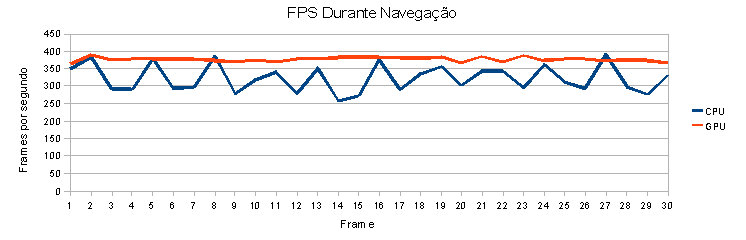
\includegraphics[width=0.9\linewidth]{img/tempoFPS.png}}
	\caption{\label{fig:fps} Gr�fico com o FPS na navega��o pelo mundo durante 30 segundos.}
\end{figure}


Como pode ser visto atrav�s do gr�fico, a navega��o pelo mundo, utilizando a gera��o dos terrenos na GPU, � muito mais fluida, sem quedas bruscas de \emph{FPS}, como nos \emph{frames} 3, 6, 9, 12, 14, 17, 20, 23, 26 e 29, gra�as �s centenas de unidades de processamento presentes na GPU.

Na gera��o pela CPU, tais quedas correspondem justamente aos momentos em que o sistema gera novos terrenos e podem resultar em um menor senso de imers�o do usu�rio no mundo virtual.